% Sångtext till VN:s sångbok 2018.

% Denna fil kan användas som sådan, bara verserna,
% namnen och annan rådata behöver bytas ur fälten.
% Tecknet "%" markerar en kommentar som helt och 
% hållet ignoreras av programmet som läser filen.

\beginsong{Punschen kommer}[				% Författare
	sr={Vals ur Glada änkan}]						% sångnamn
	

\beginverse*						% Börja vers
Punschen kommer,
punschen kommer
ljuv och sval.
Glasen imma,
röster stimma,
i vår sal.
Skål för glada minnen,
skål för varje vår.
Inga sorger finnes mer när punsch vi får!
\endverse							% Sluta vers

\endsong							% Sluta sång

\begin{intersong}
\begin{center}
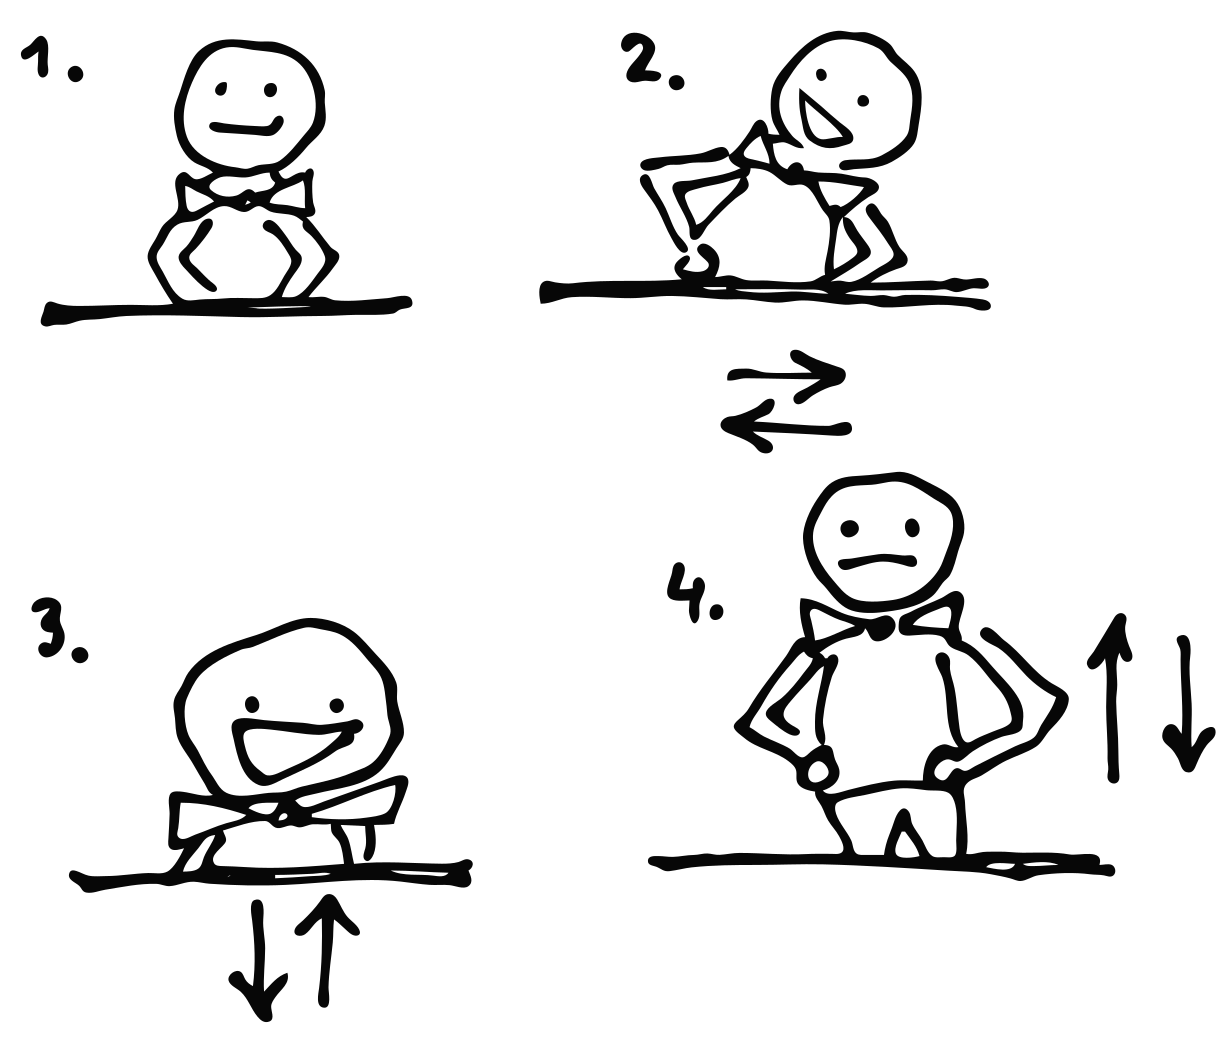
\includegraphics[scale=.5]{../bilder/punschenkommer.jpg} 
\end{center}
\end{intersong}